\subsection{Křivky}
Křivky dělíme na: \textbf{rovinné}, \textbf{prostorové}, \textbf{interpolační}, \textbf{aproximační}.

V počítači jsou reprezentovány jako soustava parametrů nějaké rovnice, která je posléze generativně zobrazována. Toto vyjádření může být v podstatě trojího druhu:
\begin{itemize}
	\item \textbf{explicitní} -- $y = f(x)$  kde  $x \quad \varepsilon \quad  \mathbb{I}$.,\\ např. $y = x^{2} + x + 1$, jedná se o parabolu.
	\item \textbf{implicitní} -- $F(x, y) = 0$, \\		$(x+9)^{2} +(y −2)^{2} −4 = 0$, kružnice se středem $[−9, 2]$ a $r=2$.
	\item \textbf{parametrické} -- 		
	\begin{equation*}
				x = f_x(t), \quad y= f_y(t), \quad z = f_z(t), parametr \quad t \quad \varepsilon <a, b>.
		\end{equation*}
		\\		$x = t, y = t^{2}, kde \quad t \quad \varepsilon \quad \mathbb{R}$, parabola s vrcholem v počátku.
		\item Jednoduchý příklad křivky je například kružnice nebo přímka.
\end{itemize}

\subsection{Parametrické křivky}
\begin{itemize}
	\item Mějme interval $I = <a, b> \subseteq \mathbb{R}$.
	\item Parametricky vyjádřenou (parametrizovanou) křivku $k$ v $\mathbb{R}^n$ nazýváme diferencovatelné zobrazení $\varphi$  :$I \rightarrow \mathbb{R}^n$
\begin{figure}[H]
\centering
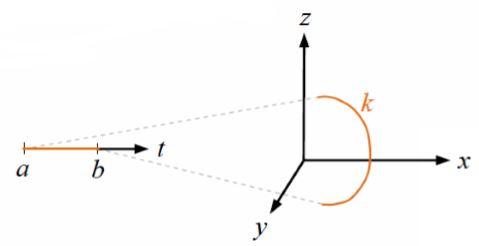
\includegraphics[width=0.5\textwidth]{assets/3_param_curve}
\end{figure}
	\item V trojrozměrném euklidovském prostoru každému číslo $t$ odpovídá na křivce příslušný bod $P(t) = [x(t), y(t), z(t)]$.
	\item Polohový vektor \textbf{P} (vektor daný počátkem souřadné soustavy a souřadnicemi příslušného bodu $P$).
\end{itemize}

\subsection{Interpolační křivky}
\begin{itemize}
	\item V PG nám pro definování (kreslení) křivky slouží její interpolace.
	\item Interpolační křivka k dané množině bodů je taková křivka, která jimi prochází.
	\item Obecně se dá křivka pro n bodů vyjádřit polynomem n1 řádu. To znamená, najít řešení soustavy pro každé:
	\begin{equation*}  
			\begin{array}{c}
			  x_{0},x_{1},...,x_{n},  \quad \quad x_{i} \neq x_{j} \quad pro  i \neq j,
			  \end{array}
			\end{equation*}
			Hledáme interpolační polynom $P_{n}(x)$ stupně nejvýše $n$, který splňuje interpolační podmínky
			\begin{equation*}  
			\begin{array}{c}
			  P_{n}(x_{i}) = y_{j} \quad \quad i = 0,1,...,n.
			  \end{array}
			\end{equation*}
	\end{itemize}

\subsection{Fergusonova křivka}
\begin{itemize}
	\item Křivka je pojmenovaná po James C. Ferguson z The Boeing Company.
	\item Je generování křivek \textbf{řízené dvěma body} a \textbf{vektory} v nich.
	\item \textbf{Hermitova interpolace} aplikovaná na složky vektorového vyjádření křivky pro jednotkovou změnu parametru na obloucích, získáme tzv. \textbf{Fergusonovy křivky}.
\end{itemize}

Ve vztahu obecně: \\
\begin{equation*} 
R(t) = F_{0}(t) G + F_{1}(t) H + F_{2}(t) g + F_{3}(t) h,
\end{equation*}
kde: F, G jsou polohové vektory bodů,\\ g,h jsou vektory tečen v bodech, ve kterých je Fergusonova křivka jednoznačně určena,\\
pro $F_{i}(t), i = 0, 1, 2, 3,$ platí: \\
\begin{equation*} 
\begin{array}{c}
F_{0}(t) = 2 t^{3} - 3t^{2} + 1, \\
F_{1}(t) = -2t^{3} + 3t^{2}, \\
F_{2}(t) = t^{3} - 2t^{2} + t, \\
F_{3}(t) = t^{3} - t^{2},  t \varepsilon <0, 1>.
\end{array}
\end{equation*}
Výsledný tvar Fergusonovy kubiky, lze ovlivnit třemi způsoby:
\begin{itemize}
	\item polohou řídících bodů $V_0$ a $V_1$,
	\item směrem tečných vektorů $v_0$ a $v_1$,
	\item velikostí tečných vektorů $v_0$ a $v_1$.
\end{itemize}
Velikost vektorů $v_0$ a $v_1$ významně ovlivňuje výsledný tvar křivky. Čím délka tečných vektorů je větší, tím více se křivka přimyká k příslušnému tečnému vektoru.
\begin{figure}[H]
\centering
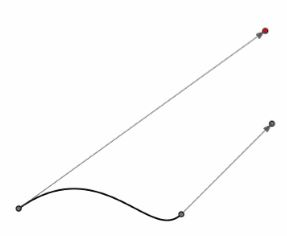
\includegraphics[width=0.4\textwidth]{assets/3_ferg_krivka}
\end{figure}
\begin{figure}[H]
\centering
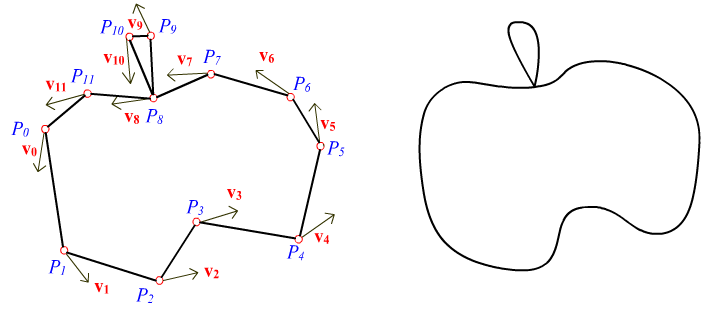
\includegraphics[width=0.5\textwidth]{assets/3_ferg_spline}
\caption{Spline}
\end{figure}


\subsection{Aproximační přímky}
\begin{itemize}
\item Někdy není možné body proložit funkcí a proto se využívá aproximačních křivek, které procházejí v blízkosti bodů.
\item Je dáno $n$ bodů. Úlohou je nalézt aproximační funkci, která nemusí procházet danými body, ale která co nejlépe vystihuje funkční závislost. 
\item Metoda nejmenších čtverců. 
			\begin{equation}
			\label{rovnicePrimky} 
			  f: y = ax + b.
			\end{equation}
			Cílem metody je dosáhnout co nejmenší počet kvadrátů euklidovského rozdělení mezi aproximovanou přímkou $f(y)$ a zadanými hodnoty $y_{i}$. Dále si nadefinujeme funci $c(a,b)$, která reprezentuje součet aproximované přímky a hodnotami $y_{i}$:
			\begin{equation}  
			\label{soucetPrimky}
			  c(a,b) = \sum_{i=0}{n} (f(x) - y_{i})^2, \\
			\end{equation}
			kde $a, b$ jsou koeficienty aproximované přímky, $n$ je počet zadaných bodů. 

			Minimum této funkce $c(a,b)$ získáme parciální derivací jejími argumenty:
			\begin{equation}  
			\label{parcialDerivation}
			  \frac{\partial c(a,b)}{\partial a} = 0,  \quad \quad  \frac{\partial c(a,b)}{\partial b} = 0
			\end{equation}
			Po vypočítání parciálních derivací získáme soustavu dvou rovnic o dvou neznýmých a dopočítáme a,b. Tyto koeficienty budou reprezentovat nalezenou aproximaci přímky, kde funkce $c(a,b)$ je nejmenší.
			\subsubsection*{Příklad}
			Zadání : \\
			\begin{equation*}  
			 A[1,1], \quad B[3,2], \quad C[2,3].
			\end{equation*}
			Nyní tyto body dosadíme do \eqref{rovnicePrimky} a získáme vzdálenost mezi zadaným bodem a aproximovanou přímkou.
			\begin{equation*}  
			1 = a + b,\\
			2 = 3a + b,\\
			3 = 2a + b,\\
			\end{equation*}
			Nyní tuto soustavu rovnic můžeme dosadit do vzorce \eqref{soucetPrimky}:
			\begin{equation*}  
			  c(a,b) = (a + b - 1)^2 + (3a + b - 2)^2 + (2a + b - 3)^2.
			\end{equation*}
			Nyní funkci parciálně derivujeme dle [\ref{parcialDerivation}]
			\begin{equation*}  
			\begin{array}{c}
			  \frac{\partial c(a,b)}{\partial a} =  2(a + b - 1) + 2(3a + b - 2)3 + 2(2a + b - 3) \quad = 28a + 12b - 26 \\
			  \frac{\partial c(a,b)}{\partial b} =  2(a + b - 1) + 2(3a + b - 2) + 2(2a + b - 3)  \quad = 12a + 6b - 12
			  \end{array}
			\end{equation*}
			Nyní vyřešíme soustavu rovnic a získáme koeficienty aproximované přímky:
			\begin{equation*}  
			\begin{array}{c}
			28a + 12b - 26 = 0 \\
			 12a + 6b - 12 = 0
			2a+1 = 0 \\
			a = - \frac{1}{2} \quad \quad b = 3
			\end{array}
			\end{equation*}
			Našli jsme aproximaci:
			\begin{equation*}  
			f : y = - \frac{1}{2} x + 3.
			\end{equation*}
			Pokud provedeme derivaci této přímky, dostaneme  $-\frac{1}{2}$. Tato hodnota je taky nazývána jako směrnice přímky a je rovna tangentě mezi přímkou a mezi kladnou poloosou x neboli nám říká, jaký je úhel mezi přímkou a poloosou x. V příloze nalezneme obrázek k tomuto příkladu.

\item Bezierova -- pomocí algoritmu Casteljau (změna parametru $t$) , Kubický Coonsův B--spline, NURBS

\end{itemize}
\subsection{Plochy}
\begin{itemize}
	\item \textbf{Rozšířením křivek} se dostaneme k plochám, které mají však s křivkami hodně společného. Zejména některé vznikly rozšířením křivek (Bezier, NURBS).
\end{itemize}
Vyjádření ploch:
\begin{itemize}
	\item \textbf{explicitní} -- $z = f(x, y)$,
	\item \textbf{implicitní} -- $F(x, y, z) = 0$,
	\item \textbf{parametrické} -- 		
	\begin{equation*}
				x = f_x(u, v), y = f_y(u, v), z = f_z(u, v). .
	\end{equation*}
\end{itemize}
\begin{itemize}
	\item Z parametrického vyjádření je snadné získat jednotlivé body, z implicitního můžeme jednoduše testovat, zda bod patří do plochy nebo ne. 
	\item \textbf{Nejvyužívanější} plochy jsou \textbf{parametrické}. 
	\item Plochy mohou být zadány \textbf{analytickým předpisem}, \textbf{hraničními křivkami}, \textbf{sítí bodů} (NURBS, Bezier) nebo plochy vytvořené \textbf{kinematicky} (rotační plochy, plochy vzniklé skládáním pohybu).
\end{itemize}
Tečné vektory plochy:
\begin{figure}[H]
\centering
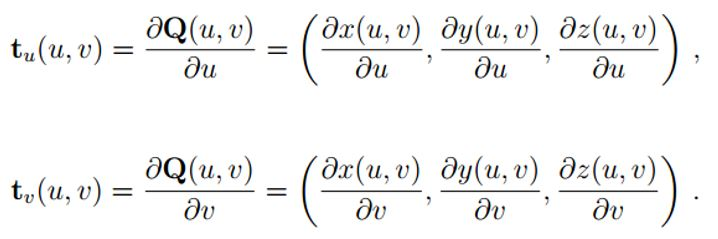
\includegraphics[width=0.6\textwidth]{assets/3_tecne_vektory_plochy}
\end{figure}
Tečná rovina:
\begin{figure}[H]
\centering
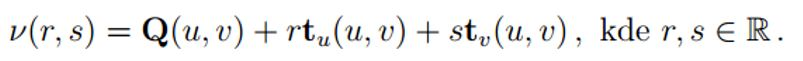
\includegraphics[width=0.7\textwidth]{assets/3_tecna_rovina}
\end{figure}

\subsection{Tečný a normálový vektor}
\subsubsection*{Tečna a tečný vektor}
\begin{itemize}
	\item Parametricky vyjádřená přímka $P(t) = (x(t), y(t), z(t))$
	\item \textbf{Tečný vektor} v bodě $t=t_0$ je dán jako $P'(t_0) = \frac{dP}{dt}(t_0) = (x'(t_0), y'(t_0), z'(t_0))$
	\item \textbf{Tečna} (přímka, která se v daném bodě křivky dotýká) je dána bodem dotyku a tečným vektorem. $Q(u) = P(t_0) + uP'(t_0)$, kde $u \varepsilon \mathbb{R}$
	\item Tečna je limitní polohou sečny, kdy oba průsečíky splynou v jeden.
\end{itemize}
\begin{itemize}
	\item \textbf{Normálový vektor} je \textbf{kolmý} na tečný vektor. Skalární součin je tedy roven 0. Potřebujeme ho pro \textbf{obecnou rovnici} přímky/roviny. Získáme jej \textbf{prohozením souřadnic směrového vektoru} a u jedné souřadnice změníme znaménko.
\end{itemize}
\subsection{Křivosti}
Křivost křivky je jedna ze \textbf{základních vlastností}, které charakterizují křivky. Rozlišujeme dva typy křivostí:
\begin{itemize}
	\item \textbf{první křivost (flexe)} -- obvykle označována pojmem \uv{křivost} a udává velikost odchýlení od křivky $P(t)$ v daném bodě $P(t_0)$. V inflexních bodech je křivost nulová.
		\begin{equation*}
				k_1(t) = \frac{|P'(t) \times P''(t)|}{|P'(t)|^3}
	\end{equation*}
	\item \textbf{druhá křivost (torze)} -– je mírou odchýlení křivky $P(t)$ v daném bodě $P(t_0)$ z její oskulační roviny (viz. oskulační rovina) do prostoru.
	\begin{equation*}
				k_2(t) = \frac{(P'(t) \times P''(t)) \cdot P'''(t)}{|P'(t) \times P''(t)|^2}
	\end{equation*}
\end{itemize}
\subsubsection{Oskulační rovina}
Každá rovina procházející tečnou křivky v bodě $P(t0)$ se nazývá \textbf{tečná rovina}. Oskulační rovina je \textbf{limitní rovinou} těchto rovin. Pomocí bodu $P(t0)$ a dvou vektorů $P'(t0)$ a$ P''(t0)$ zjistíme oskulační rovinu. Jsou--li tyto dva vektory lineárně nezávislé, existuje právě jedna oskulační rovina v daném bodě. V opačném případě je oskulační rovinou každá tečná rovina.

\subsection{Cn a Gn Spojitost}
\begin{itemize}
\item Při navazování oblouků je významným faktorem spojitost křivek. 
\item Výsledná křivka je \textbf{spojitá}, pokud je spojitá \textbf{ve všech svých bodech}, a tedy zejména v navazovacích bodech. 
\item Křivka je \textbf{hladká}, pokud jsou ve všech jejích bodech \textbf{spojité i její první derivace}. Pro vyšší derivace říkáme, že křivka má spojitost druhého, třetího a obecně $n$--tého řádu.
\item Význam spojitosti křivek:
	\begin{itemize}
	\item vizuální stránka napojení dvou křivek,
	\item animace křivky.
	\end{itemize}
\end{itemize}
$\mathbf{C_n}$ -- parametrická spojitost:
	\begin{itemize}
	\item $\mathbf{c_0}$ -- koncový bod prvního segmentu je počátečním bodem segmentu druhého,	
	\item $\mathbf{c_1}$ -- rovnost tečných vektorů v daném uzlu, 		
	\item $\mathbf{c_2}$ -- rovnost prvních derivací tečných vektorů v daném uzlu.
	\end{itemize}
Čím vyšší spojitost je požadována, tím delší "dobu" (ve smyslu parametru $\mathbf{t}$) se oba segmenty k sobě přimykají. Ze spojitosti $\mathbf{c_0}$ plyne, že bod se pohybuje po spojité dráze, ale v uzlu může měnit skokem směr pohybu, rychlost i zrychlení. Směr pohybu a velikost rychlosti se nemůže měnit skokem při spojitosti $\mathbf{c_1}$ a zrychlení zůstává nezměněné při spojitosti $\mathbf{c_2}$. \\\\
$\mathbf{G_n}$ -- geometrická spojitost:
	\begin{itemize}
		\item $\mathbf{g_0}$ -- koncový bod prvního segmentu je počátečním bodem segmentu druhého
		\item $\mathbf{g_1}$ -- tečné vektory jsou lineárně závislé
	\end{itemize}
Opticky zaručuje $\mathbf{g_1}$ spojitost "skoro stejnou" hladkost jako $\mathbf{c_1}$. Z hlediska použití bývá jednodušší zaručit spojitost $\mathbf{g_1}$ nežli $\mathbf{c_1}$.

\subsection{Bézier}
\begin{itemize}
	\item Pierre Étienne Bézier (1910 - 1999) Renault
	\item mějme zadání $n + 1$ řídících bodů $P_0, P_1,...,P_n$, kde $n \geq 1$.
	\item Bézierova křivka je zadána jako
			\begin{equation*} 
			P(t) = \sum\limits_{k=0}^n P_{i} B_{i}^{n}(t),
			\end{equation*}
			kde: $t \varepsilon <0,1>$, $P_{i}$ je počet bodů a $B_{i}^{n}(t)$ reprezentuje Bersteinovy polynomy. 
	\item Pro výpočet bázových funkcí se využívá Bersteinových polynomů:
			\begin{equation*} 
			B_{i}^{n}(t) = \binom{n}{i} t^{i} (t - 1)^{n-i},
			\end{equation*}
			kde: $t \varepsilon <0,1>$, $n$ je polynomiální stupeň (počet bodů), $i$ je index a $t$ parametr. 
	\item Jednoduchá Bézierová křivka je přímka z bodu $P_{0}$ do bodu $P_{1}$.
	\item Kvadratická Bézierová křivka je definována třemi kontrolními body.
	\item Kubická Bézierová křivka je definována čtyřmi kontrolními body $P_{0}$, $P_{1}$, $P_{2}$ a $P_{3}$. \\
	Body $P_{0}$, $P_{2}$ a tyto tečné vektory dosadíme do vzorce: 
	\begin{equation*} 
	P(t) = P_{0} \binom{3}{0} t^{0} (t - 1)^{3} + P_{1} \binom{3}{1} t^{1} (t - 1)^{2} + P_{2} \binom{3}{2} t^{2} (t - 1)^{1} + P_{3} \binom{3}{3} t^{3} (t - 1)^{0}
	\end{equation*}
\end{itemize}

\subsubsection*{Konstrukce Bézierovy křivky}
\begin{figure}[H]
\centering
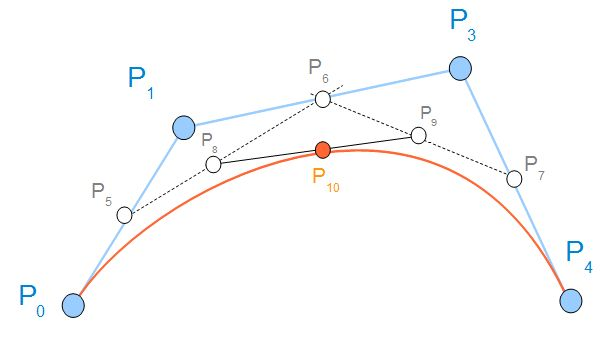
\includegraphics[width=0.5\textwidth]{assets/2_bezier_ex}
\end{figure}
Pro geometrickou konstrukci Beziérovy křivky zvolíme poměr t v kterém dělíme lomenou řídící čáru, jak je vidět na obrázku nahoře, kde je $t=0,5$. 

Takto jsme vykreslili první bod křivky $\mathbf{P_10}$. Konstrukcí bodu $\mathbf{P_10}$ jsme získali nové řídící body, které použijeme pro získání dalších bodů křivky. Další dva body křivky tedy získáme stejným způsobem za použití řídících bodů {$\mathbf{P_0}$, $\mathbf{P_5}$, $\mathbf{P_8}$, $\mathbf{P_10}$} a {$\mathbf{P_10}$, $\mathbf{P_9}$, $\mathbf{P_7}$, $\mathbf{P_4}$}. Tímto rekurzivním způsobem postupně vykreslíme celou křivku.

Výhoda této konstrukce je, že můžeme ovlivnit hustotu vykreslování dle potřeby. Například v oblasti velkého zakřivení.

\subsubsection*{Převod Fergusonovy kubiky na Beziérovu kubika}
Fergusonovu křivku lze převést na Beziérovu křivku, pokud se budeme při výpočtu držet následujícího pravidla:
	\begin{equation*} 
	\begin{array}{c}
	P_0 = V_0,\\
	P_1 = V_0 + \frac{1}{3}\vec{u},\\
	P_2 = V_1 − \frac{1}{3}\vec{v},\\
	P_3 = V_1.
	\end{array}
	\end{equation*}


\subsection{Coons}
\begin{itemize}
	\item Coonsnová kubická B-spline křivka vznikne pospojováním Connsnových kubik, tak aby byla zajištěna spojitost druhého řádu.
	\item Coonsnová kubika je parametrická křivka dána čtyřmi body $P_0, P_1, P_2, P_3$ a tímto vztahem:
		\begin{equation*} 
			P(t) = \frac{1}{6} (P_0C_0(t) + P_1C_1(t) + P_2C_2(t) + P_3C_3(t))
		\end{equation*}
		kde bázové funkce jsou:
		\begin{equation*} 
		\begin{array}{c}
			C_0(t) = -t^3 + 3t^2 - 3t + 1, \\
			C_1(t) = 3t^3 + 6t^2 + 4, \\
			C_2(t) = -3t^3 + 3t^2 + 3t + 1, \\
			C_3(t) = t^3
		\end{array}		
		\end{equation*}
\end{itemize}
\begin{figure}[H]
\centering
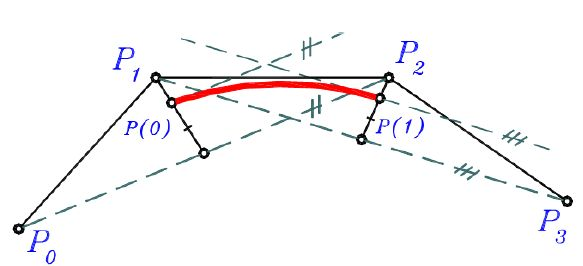
\includegraphics[width=0.7\textwidth]{assets/2_coons-b-spline}
\end{figure}
\subsection{NURBS}
\begin{itemize}
	\item Non-uniform rational basis spline (NURBS)
	%našel jsem toto, ale jak jsem viděl ty vzorce, meh, nechtělo se mi to ani dělat :D
	% https://www.root.cz/clanky/krivky-nurbs-1/
\end{itemize}